\section{PROPOSED FRAMEWORK}
\label{sec:framework}
\begin{figure}
    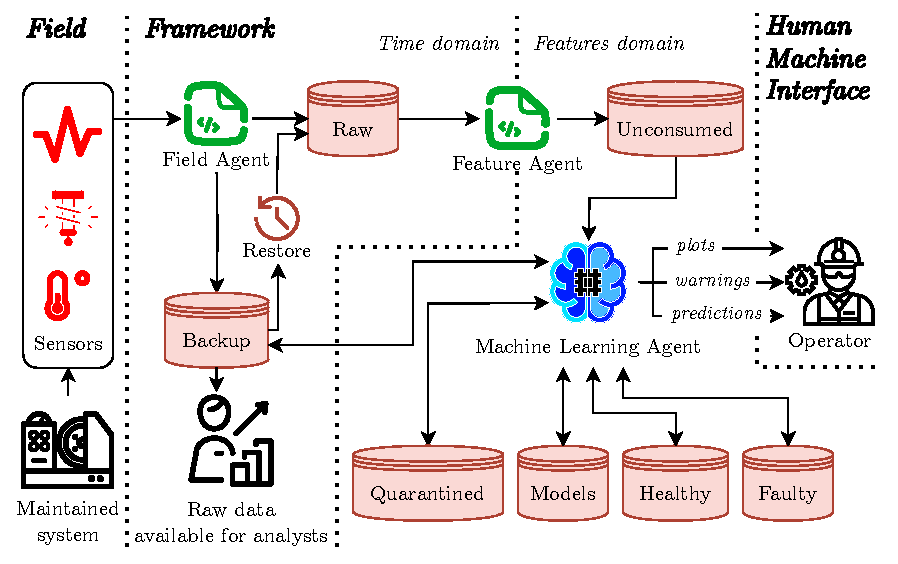
\includegraphics[width=\linewidth]{images/Framework_structure.pdf}
    \caption{The structure of the proposed framework. The Field Agent collects the time series, the Feature Agent extracts the features, and the Machine Learning Agent evaluates the health of the maintained device. The agents are connected to collections of a common database. The 
\includegraphics[height = 1em]{images/DB_icon-cropped.pdf} icon represents a collection of a database that every agent can read and write.}
    \label{fig:framework_structure}
\end{figure}

The solution developed in this thesis is thought to be set up on a new device, and linked to the signals of the most informative sensors of the system.
In the first phase of commissioning, the framework collects the data, extracts the features and stores them. When the collected data are enough to characterize all the modes of operation of the maintained system, the UML model can be trained. Finally, the framework continues collecting new time series, extracting the features and evaluating these new samples. Now, the framework produces a Novelty Metric (NM) that quantifies how anomalous the new data are. 
This phase lasts indefinitely (until the maintenance team performs a model update). When the NM overshoots a certain threshold, a warning is issued to the maintenance team. 
Then, the team can decide to perform a maintenance action or to continue monitoring the system. If the team declares the system as healthy, the framework can be retrained with the new data, to update the UML model. Otherwise, the framework can be trained to characterize also the newly discovered fault in order to perform Fault Detection (FD) in the future.

\subsection{Software Agents}
The proposed framework is based on software agents. Each agent is autonomous and performs a specific task. The developed agents, as shown in Fig.~\ref{fig:framework_structure}, are:
\begin{itemize}
    \item \textbf{Field Agent (FiA)}: responsible for the synchronous sampling of the data. It provides the time series records and ensures a correct sampling frequency.
    \item \textbf{Feature Agent (FA)}: extracts the features from the time series.
    \item \textbf{Machine Learning Agent (MLA)}: trains the UML algorithms and then performs ND, FD and PM. It reports the results to the user.
\end{itemize}

\subsection{Database}
{
All the Agents are connected to different collections of a common database. In the case of the PC implementation, MongoDB has been used. In the case of the Edge implemen- tation the data are stored directly in the microcontroller's memory.
Regarding the structure shown in Fig.~\ref{fig:framework_structure}, the MongoDB database is composed of seven collections. Every collection has a specific role in the framework. For example, the \emph{Quarantined, Healthy} and \emph{Faulty} collections contain the features that have been flagged as novelty, normal or faulty, respectively.
}

\subsection{Multiple Instances}
As shown in Fig.~\ref{fig:multiple_instances}, multiple instances of the framework can be implemented to better isolate the location of the anomaly in a complex system. The larger the set of sensors that a single instance of the framework is connected to, the more difficult it is to isolate the anomaly. On the other hand, configuring a large group of sensors allows the detection of complex anomalies. 

For example, a shaft with two bearings can be monitored by two instances of the framework, one for each bearing vibration signal. Another instance can be linked to the signals of both bearings to detect more complex novelty patterns that are not detectable by analyzing the signals separately.   

\begin{figure}
    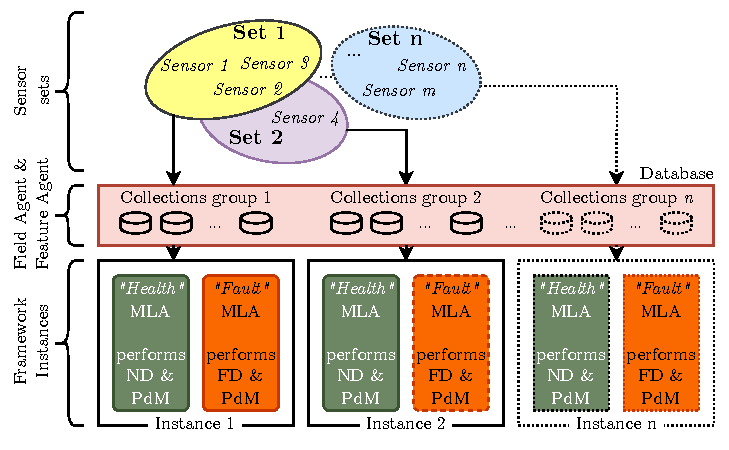
\includegraphics[width=\linewidth]{images/FrameworkInstances.pdf}
    \caption{Multiple instances implementation of the framework. Every instance is linked to a different set of sensors, to monitor different parts of the system.}
    \label{fig:multiple_instances}
\end{figure}


\subsection{Unsupervised Machine Learning Models}

The UML implemented in the framework are: \emph{K-means}, \emph{DBSCAN}, \emph{Gaussian Mixture Model} (GMM), \emph{Isolation Forest} (IF), \emph{Local Outlier Factor} (LOF), \emph{One-Class Support Vector Machine} ($\nu$-SVM).

K-means and DBSCAN are traditionally clustering algorithms, so a custom NM has been developed for these algorithms. For example, if K-means is used, the NM is defined as the distance of a sample from the closest centroid, normalized by the cluster radius. The other models are already commonly used for ND, so the NM has been linked to the \quoted{score} provided by the library functions.

If the UML is trained with faulty data, instead of normal ones, then it performs FD. The NM measures \quoted{how not faulty} the new data are. In this case, the value is transformed into a Fault Metric (FM) with the function $\text{FM} = - \ln(\text{NM} + 1)$ to preserve the coherence (the lower the metric, the healthier the system). 